\documentclass[10pt]{beamer}

\usetheme[progressbar=frametitle]{metropolis}
\usepackage{appendixnumberbeamer}

\usepackage{booktabs}

%For linking email and website
\usepackage{hyperref}

% For \coloneqq
\usepackage{mathtools}

%For enumeration as words
\usepackage{blindtext}
\usepackage{enumerate}

\usepackage{multirow}

\usepackage{xspace}
\newcommand{\themename}{\textbf{\textsc{metropolis}}\xspace}

\newcommand{\codeB}[1]{\texttt{#1}}


\title{Theory of Computation}
\subtitle{Tutorial - NFAs}
\date{}
\author{Cesare Spinoso-Di Piano}

\begin{document}

\maketitle

\begin{frame}{Plan for today}
    \setbeamertemplate{section in toc}[sections numbered]
    \tableofcontents[hideallsubsections]
\end{frame}


\section{NFAs}

\begin{frame}{NFAs}

\end{frame}

\begin{frame}[t]{Formal definition of an NFA}
    \textbf{Definition.} A \textbf{\underline{nondeterministic} finite automaton (NFA)} $M$ is a 5 element tuple $M = (Q, \Sigma, \delta, q_0, F)$ where
    \begin{itemize}
        \item $Q$ is the set of all states
        \item $\Sigma$ is the alphabet
        \item \textcolor{red}{*} $\delta$ is the transition function $\delta: Q \times \{\Sigma \cup \{\lambda\} \} \rightarrow 2^Q$
        \item $q_0$ is the (\underline{unique}) initial state
        \item $F$ is the set of final states
    \end{itemize}
    An NFA is a machine that reads an input string and either accepts it or rejects it.

    \textcolor{red}{*\textbf{Unlike a DFA: }}
    The transition function of an NFA can accept $\lambda$ and \textbf{always} returns a set.
\end{frame}


\begin{frame}{NFAs as language accepters}
    \textbf{Non-Determinism.} Let $N$ be an NFA with input string $w$. Non-determinism allows $N$ to try \textit{all possible walks}. If at least one walk leads to a final state, then $N$ accepts $w$.

    \textbf{Definition.} Formally, given an NFA $N$ the language accepted by $N$ is
    \[
        L(N) = \{w \in \Sigma ^*: \delta^*(q_0, w) \cap F \neq \emptyset\}
    \]
    where $\delta^*$ is the extended transition function $\delta^*: Q \times \Sigma^* \rightarrow 2^Q$.
\end{frame}


\begin{frame}{Example}
    \textbf{Example.} Consider the following NFA over the alphabet $\Sigma = \{a\}$.

    \begin{center}
        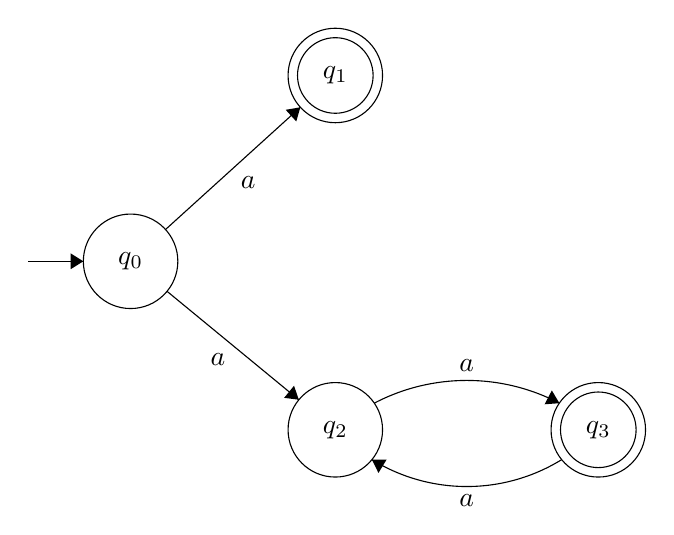
\begin{tikzpicture}[scale=0.2]
            \tikzstyle{every node}+=[inner sep=0pt]
            \draw [black] (8.9,-29.1) circle (3);
            \draw (8.9,-29.1) node {$q_0$};
            \draw [black] (21.9,-17.3) circle (3);
            \draw (21.9,-17.3) node {$q_1$};
            \draw [black] (21.9,-17.3) circle (2.4);
            \draw [black] (21.9,-39.8) circle (3);
            \draw (21.9,-39.8) node {$q_2$};
            \draw [black] (38.6,-39.8) circle (3);
            \draw (38.6,-39.8) node {$q_3$};
            \draw [black] (38.6,-39.8) circle (2.4);
            \draw [black] (2.4,-29.1) -- (5.9,-29.1);
            \fill [black] (5.9,-29.1) -- (5.1,-28.6) -- (5.1,-29.6);
            \draw [black] (11.12,-27.08) -- (19.68,-19.32);
            \fill [black] (19.68,-19.32) -- (18.75,-19.48) -- (19.42,-20.22);
            \draw (16.36,-23.69) node [below] {$a$};
            \draw [black] (11.22,-31.01) -- (19.58,-37.89);
            \fill [black] (19.58,-37.89) -- (19.28,-37) -- (18.65,-37.77);
            \draw (14.45,-34.94) node [below] {$a$};
            \draw [black] (24.37,-38.109) arc (117.6149:62.3851:12.686);
            \fill [black] (36.13,-38.11) -- (35.65,-37.3) -- (35.19,-38.18);
            \draw (30.25,-36.16) node [above] {$a$};
            \draw [black] (36.281,-41.69) arc (-58.29883:-121.70117:11.478);
            \fill [black] (24.22,-41.69) -- (24.64,-42.54) -- (25.16,-41.69);
            \draw (30.25,-43.9) node [below] {$a$};
        \end{tikzpicture}
    \end{center}

\end{frame}

\begin{frame}{Example - Tracing Input}
    \textbf{Input String: \textcolor{red}{\^{}}aa}

    \begin{center}
        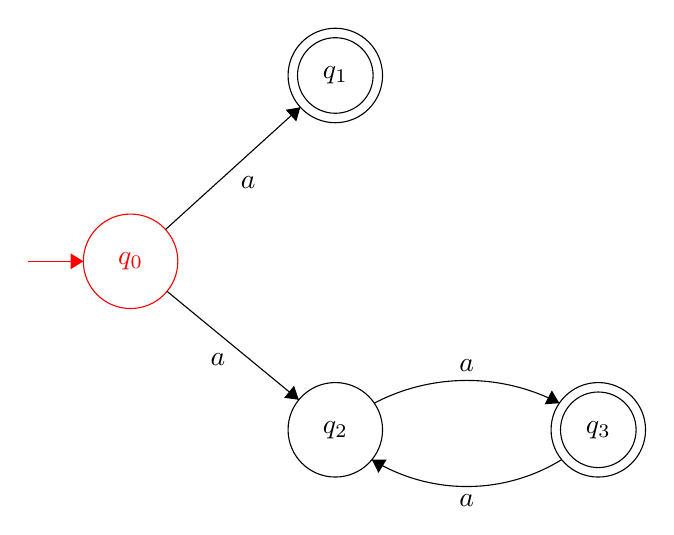
\begin{tikzpicture}[scale=0.2]
            \tikzstyle{every node}+=[inner sep=0pt]
            \draw [red] (8.9,-29.1) circle (3);
            \draw [red] (8.9,-29.1) node {$q_0$};
            \draw [red] [black] (21.9,-17.3) circle (3);
            \draw (21.9,-17.3) node {$q_1$};
            \draw [black] (21.9,-17.3) circle (2.4);
            \draw [black] (21.9,-39.8) circle (3);
            \draw (21.9,-39.8) node {$q_2$};
            \draw [black] (38.6,-39.8) circle (3);
            \draw (38.6,-39.8) node {$q_3$};
            \draw [black] (38.6,-39.8) circle (2.4);
            \draw [red] (2.4,-29.1) -- (5.9,-29.1);
            \fill [red] (5.9,-29.1) -- (5.1,-28.6) -- (5.1,-29.6);
            \draw [black] (11.12,-27.08) -- (19.68,-19.32);
            \fill [black] (19.68,-19.32) -- (18.75,-19.48) -- (19.42,-20.22);
            \draw (16.36,-23.69) node [below] {$a$};
            \draw [black] (11.22,-31.01) -- (19.58,-37.89);
            \fill [black] (19.58,-37.89) -- (19.28,-37) -- (18.65,-37.77);
            \draw (14.45,-34.94) node [below] {$a$};
            \draw [black] (24.37,-38.109) arc (117.6149:62.3851:12.686);
            \fill [black] (36.13,-38.11) -- (35.65,-37.3) -- (35.19,-38.18);
            \draw (30.25,-36.16) node [above] {$a$};
            \draw [black] (36.281,-41.69) arc (-58.29883:-121.70117:11.478);
            \fill [black] (24.22,-41.69) -- (24.64,-42.54) -- (25.16,-41.69);
            \draw (30.25,-43.9) node [below] {$a$};
        \end{tikzpicture}
    \end{center}

\end{frame}

\begin{frame}{Example - Tracing Input}
    \textbf{Input String: \textcolor{red}aa}

    \begin{center}
        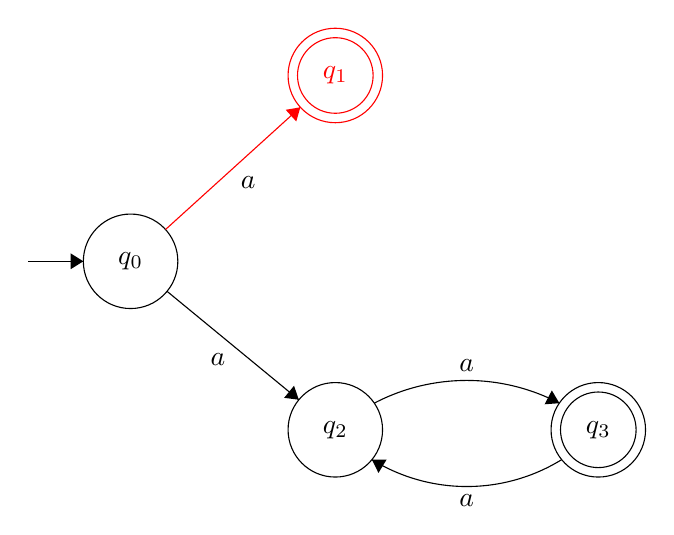
\begin{tikzpicture}[scale=0.2]
            \tikzstyle{every node}+=[inner sep=0pt]
            \draw [black] (8.9,-29.1) circle (3);
            \draw [black] (8.9,-29.1) node {$q_0$};
            \draw [red] (21.9,-17.3) circle (3);
            \draw [red] (21.9,-17.3) node {$q_1$};
            \draw [red] (21.9,-17.3) circle (2.4);
            \draw [black] (21.9,-39.8) circle (3);
            \draw (21.9,-39.8) node {$q_2$};
            \draw [black] (38.6,-39.8) circle (3);
            \draw (38.6,-39.8) node {$q_3$};
            \draw [black] (38.6,-39.8) circle (2.4);
            \draw [black] (2.4,-29.1) -- (5.9,-29.1);
            \fill [black] (5.9,-29.1) -- (5.1,-28.6) -- (5.1,-29.6);
            \draw [red] (11.12,-27.08) -- (19.68,-19.32);
            \fill [red] (19.68,-19.32) -- (18.75,-19.48) -- (19.42,-20.22);
            \draw (16.36,-23.69) node [below] {$a$};
            \draw [black] (11.22,-31.01) -- (19.58,-37.89);
            \fill [black] (19.58,-37.89) -- (19.28,-37) -- (18.65,-37.77);
            \draw (14.45,-34.94) node [below] {$a$};
            \draw [black] (24.37,-38.109) arc (117.6149:62.3851:12.686);
            \fill [black] (36.13,-38.11) -- (35.65,-37.3) -- (35.19,-38.18);
            \draw (30.25,-36.16) node [above] {$a$};
            \draw [black] (36.281,-41.69) arc (-58.29883:-121.70117:11.478);
            \fill [black] (24.22,-41.69) -- (24.64,-42.54) -- (25.16,-41.69);
            \draw (30.25,-43.9) node [below] {$a$};
        \end{tikzpicture}
    \end{center}

\end{frame}

\begin{frame}{Example - Tracing Input}
    \textbf{Input String: a\textcolor{red}a} \\
    $\delta(q_1, a) = \emptyset$, no where to go. Are we done?

    \begin{center}
        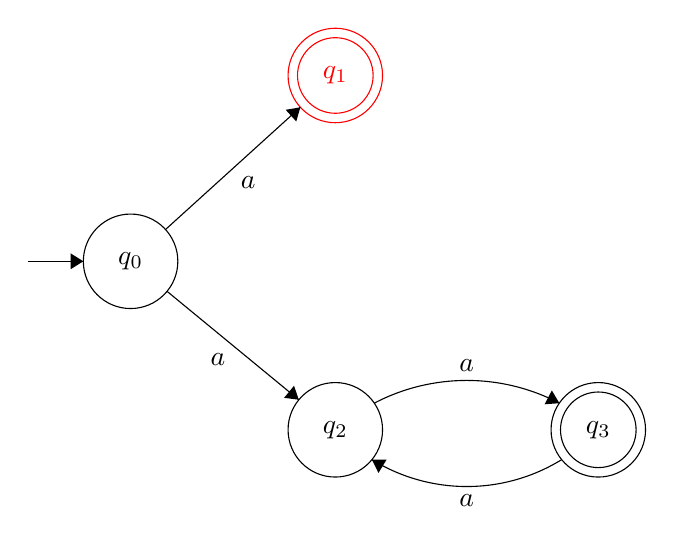
\begin{tikzpicture}[scale=0.2]
            \tikzstyle{every node}+=[inner sep=0pt]
            \draw [black] (8.9,-29.1) circle (3);
            \draw [black] (8.9,-29.1) node {$q_0$};
            \draw [red] (21.9,-17.3) circle (3);
            \draw [red] (21.9,-17.3) node {$q_1$};
            \draw [red] (21.9,-17.3) circle (2.4);
            \draw [black] (21.9,-39.8) circle (3);
            \draw (21.9,-39.8) node {$q_2$};
            \draw [black] (38.6,-39.8) circle (3);
            \draw (38.6,-39.8) node {$q_3$};
            \draw [black] (38.6,-39.8) circle (2.4);
            \draw [black] (2.4,-29.1) -- (5.9,-29.1);
            \fill [black] (5.9,-29.1) -- (5.1,-28.6) -- (5.1,-29.6);
            \draw [black] (11.12,-27.08) -- (19.68,-19.32);
            \fill [black] (19.68,-19.32) -- (18.75,-19.48) -- (19.42,-20.22);
            \draw (16.36,-23.69) node [below] {$a$};
            \draw [black] (11.22,-31.01) -- (19.58,-37.89);
            \fill [black] (19.58,-37.89) -- (19.28,-37) -- (18.65,-37.77);
            \draw (14.45,-34.94) node [below] {$a$};
            \draw [black] (24.37,-38.109) arc (117.6149:62.3851:12.686);
            \fill [black] (36.13,-38.11) -- (35.65,-37.3) -- (35.19,-38.18);
            \draw (30.25,-36.16) node [above] {$a$};
            \draw [black] (36.281,-41.69) arc (-58.29883:-121.70117:11.478);
            \fill [black] (24.22,-41.69) -- (24.64,-42.54) -- (25.16,-41.69);
            \draw (30.25,-43.9) node [below] {$a$};
        \end{tikzpicture}
    \end{center}

\end{frame}

\begin{frame}{Example - Tracing Input}
    \textbf{Input String: \textcolor{red}{\^{}}aa } \\
    Are we done? No, \textbf{M} tries another walk.

    \begin{center}
        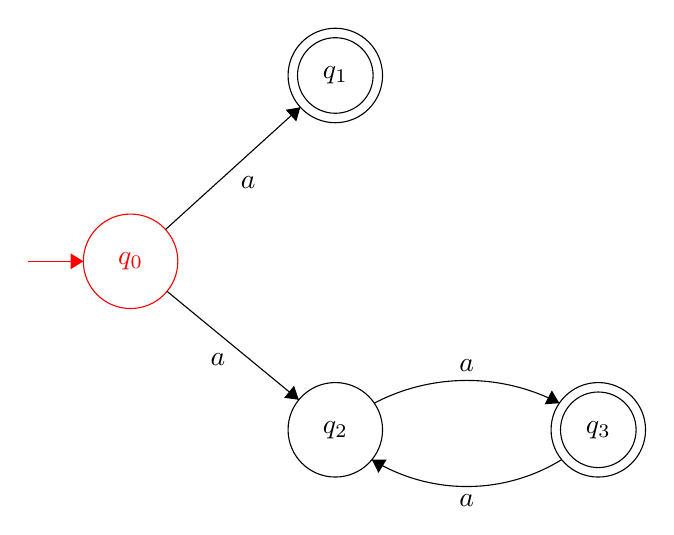
\begin{tikzpicture}[scale=0.2]
            \tikzstyle{every node}+=[inner sep=0pt]
            \draw [red] (8.9,-29.1) circle (3);
            \draw [red] (8.9,-29.1) node {$q_0$};
            \draw [red] [black] (21.9,-17.3) circle (3);
            \draw (21.9,-17.3) node {$q_1$};
            \draw [black] (21.9,-17.3) circle (2.4);
            \draw [black] (21.9,-39.8) circle (3);
            \draw (21.9,-39.8) node {$q_2$};
            \draw [black] (38.6,-39.8) circle (3);
            \draw (38.6,-39.8) node {$q_3$};
            \draw [black] (38.6,-39.8) circle (2.4);
            \draw [red] (2.4,-29.1) -- (5.9,-29.1);
            \fill [red] (5.9,-29.1) -- (5.1,-28.6) -- (5.1,-29.6);
            \draw [black] (11.12,-27.08) -- (19.68,-19.32);
            \fill [black] (19.68,-19.32) -- (18.75,-19.48) -- (19.42,-20.22);
            \draw (16.36,-23.69) node [below] {$a$};
            \draw [black] (11.22,-31.01) -- (19.58,-37.89);
            \fill [black] (19.58,-37.89) -- (19.28,-37) -- (18.65,-37.77);
            \draw (14.45,-34.94) node [below] {$a$};
            \draw [black] (24.37,-38.109) arc (117.6149:62.3851:12.686);
            \fill [black] (36.13,-38.11) -- (35.65,-37.3) -- (35.19,-38.18);
            \draw (30.25,-36.16) node [above] {$a$};
            \draw [black] (36.281,-41.69) arc (-58.29883:-121.70117:11.478);
            \fill [black] (24.22,-41.69) -- (24.64,-42.54) -- (25.16,-41.69);
            \draw (30.25,-43.9) node [below] {$a$};
        \end{tikzpicture}
    \end{center}

\end{frame}

\begin{frame}{Example - Tracing Input}
    \textbf{Input String: \textcolor{red}aa } \\

    \begin{center}
        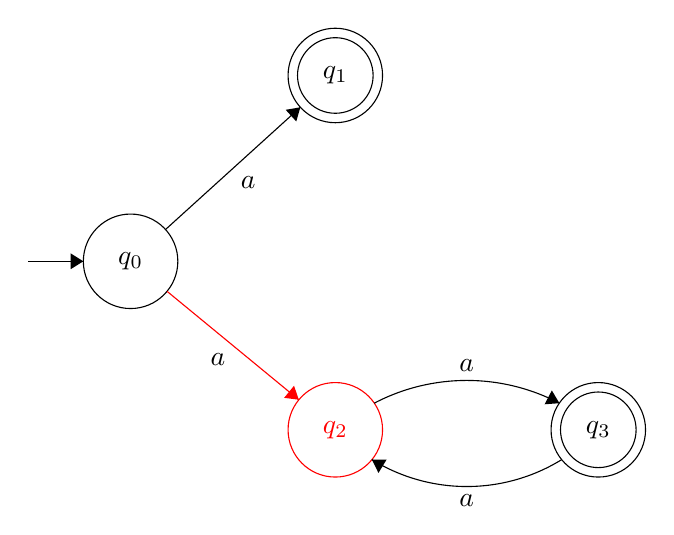
\begin{tikzpicture}[scale=0.2]
            \tikzstyle{every node}+=[inner sep=0pt]
            \draw [black] (8.9,-29.1) circle (3);
            \draw [black] (8.9,-29.1) node {$q_0$};
            \draw [black] (21.9,-17.3) circle (3);
            \draw [black] (21.9,-17.3) node {$q_1$};
            \draw [black] (21.9,-17.3) circle (2.4);
            \draw [red] (21.9,-39.8) circle (3);
            \draw [red] (21.9,-39.8) node {$q_2$};
            \draw [black] (38.6,-39.8) circle (3);
            \draw (38.6,-39.8) node {$q_3$};
            \draw [black] (38.6,-39.8) circle (2.4);
            \draw [black] (2.4,-29.1) -- (5.9,-29.1);
            \fill [black] (5.9,-29.1) -- (5.1,-28.6) -- (5.1,-29.6);
            \draw [black] (11.12,-27.08) -- (19.68,-19.32);
            \fill [black] (19.68,-19.32) -- (18.75,-19.48) -- (19.42,-20.22);
            \draw (16.36,-23.69) node [below] {$a$};
            \draw [red] (11.22,-31.01) -- (19.58,-37.89);
            \fill [red] (19.58,-37.89) -- (19.28,-37) -- (18.65,-37.77);
            \draw (14.45,-34.94) node [below] {$a$};
            \draw [black] (24.37,-38.109) arc (117.6149:62.3851:12.686);
            \fill [black] (36.13,-38.11) -- (35.65,-37.3) -- (35.19,-38.18);
            \draw (30.25,-36.16) node [above] {$a$};
            \draw [black] (36.281,-41.69) arc (-58.29883:-121.70117:11.478);
            \fill [black] (24.22,-41.69) -- (24.64,-42.54) -- (25.16,-41.69);
            \draw (30.25,-43.9) node [below] {$a$};
        \end{tikzpicture}
    \end{center}

\end{frame}



\begin{frame}{Example - Tracing Input}
    \textbf{Input String: a\textcolor{red}a } \\

    \begin{center}
        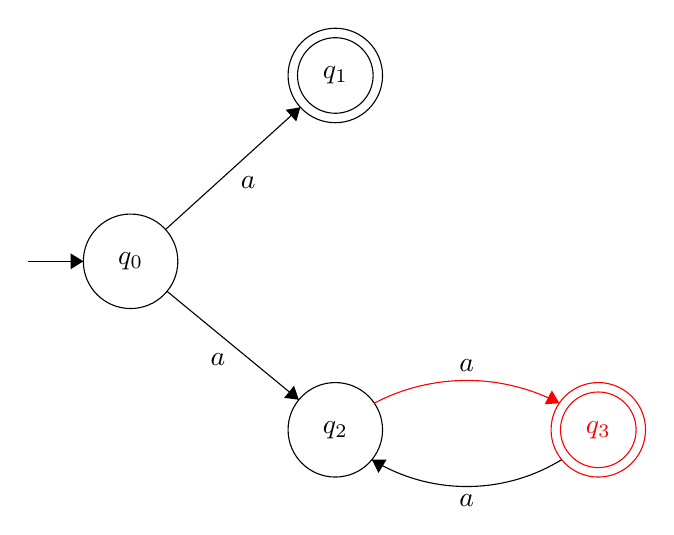
\begin{tikzpicture}[scale=0.2]
            \tikzstyle{every node}+=[inner sep=0pt]
            \draw [black] (8.9,-29.1) circle (3);
            \draw [black] (8.9,-29.1) node {$q_0$};
            \draw [black] (21.9,-17.3) circle (3);
            \draw [black] (21.9,-17.3) node {$q_1$};
            \draw [black] (21.9,-17.3) circle (2.4);
            \draw [black] (21.9,-39.8) circle (3);
            \draw [black] (21.9,-39.8) node {$q_2$};
            \draw [red] (38.6,-39.8) circle (3);
            \draw [red] (38.6,-39.8) node {$q_3$};
            \draw [red] (38.6,-39.8) circle (2.4);
            \draw [black] (2.4,-29.1) -- (5.9,-29.1);
            \fill [black] (5.9,-29.1) -- (5.1,-28.6) -- (5.1,-29.6);
            \draw [black] (11.12,-27.08) -- (19.68,-19.32);
            \fill [black] (19.68,-19.32) -- (18.75,-19.48) -- (19.42,-20.22);
            \draw (16.36,-23.69) node [below] {$a$};
            \draw [black] (11.22,-31.01) -- (19.58,-37.89);
            \fill [black] (19.58,-37.89) -- (19.28,-37) -- (18.65,-37.77);
            \draw (14.45,-34.94) node [below] {$a$};
            \draw [red] (24.37,-38.109) arc (117.6149:62.3851:12.686);
            \fill [red] (36.13,-38.11) -- (35.65,-37.3) -- (35.19,-38.18);
            \draw (30.25,-36.16) node [above] {$a$};
            \draw [black] (36.281,-41.69) arc (-58.29883:-121.70117:11.478);
            \fill [black] (24.22,-41.69) -- (24.64,-42.54) -- (25.16,-41.69);
            \draw (30.25,-43.9) node [below] {$a$};
        \end{tikzpicture}
    \end{center}

    One of the possible walks ends in a final state, \textbf{M} accepts this string.

\end{frame}

\begin{frame}{Example - Tracing Input}
    \textbf{Input String: aaa} \\

    \begin{center}
        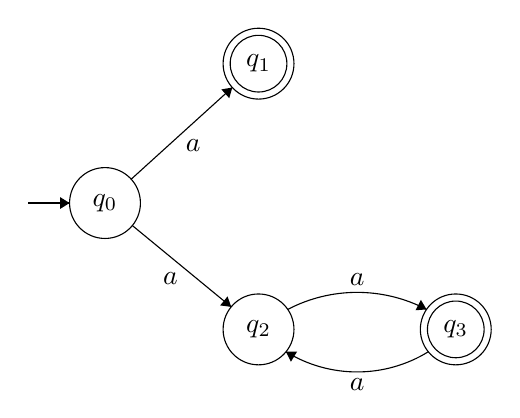
\begin{tikzpicture}[scale=0.15]
            \tikzstyle{every node}+=[inner sep=0pt]
            \draw [black] (8.9,-29.1) circle (3);
            \draw [black] (8.9,-29.1) node {$q_0$};
            \draw [black] (21.9,-17.3) circle (3);
            \draw [black] (21.9,-17.3) node {$q_1$};
            \draw [black] (21.9,-17.3) circle (2.4);
            \draw [black] (21.9,-39.8) circle (3);
            \draw [black] (21.9,-39.8) node {$q_2$};
            \draw [black] (38.6,-39.8) circle (3);
            \draw [black] (38.6,-39.8) node {$q_3$};
            \draw [black] (38.6,-39.8) circle (2.4);
            \draw [black] (2.4,-29.1) -- (5.9,-29.1);
            \fill [black] (5.9,-29.1) -- (5.1,-28.6) -- (5.1,-29.6);
            \draw [black] (11.12,-27.08) -- (19.68,-19.32);
            \fill [black] (19.68,-19.32) -- (18.75,-19.48) -- (19.42,-20.22);
            \draw (16.36,-23.69) node [below] {$a$};
            \draw [black] (11.22,-31.01) -- (19.58,-37.89);
            \fill [black] (19.58,-37.89) -- (19.28,-37) -- (18.65,-37.77);
            \draw (14.45,-34.94) node [below] {$a$};
            \draw [black] (24.37,-38.109) arc (117.6149:62.3851:12.686);
            \fill [black] (36.13,-38.11) -- (35.65,-37.3) -- (35.19,-38.18);
            \draw (30.25,-36.16) node [above] {$a$};
            \draw [black] (36.281,-41.69) arc (-58.29883:-121.70117:11.478);
            \fill [black] (24.22,-41.69) -- (24.64,-42.54) -- (25.16,-41.69);
            \draw (30.25,-43.9) node [below] {$a$};
        \end{tikzpicture}
    \end{center}

    In both traces (top and bottom), do not end up in a final state. \textbf{M} rejects this string.

    What is the language accepted by this NFA?
\end{frame}

\begin{frame}[t]{Exercise}
    \textbf{Exercise.} Given the following NFA \textbf{M},

    \begin{center}
        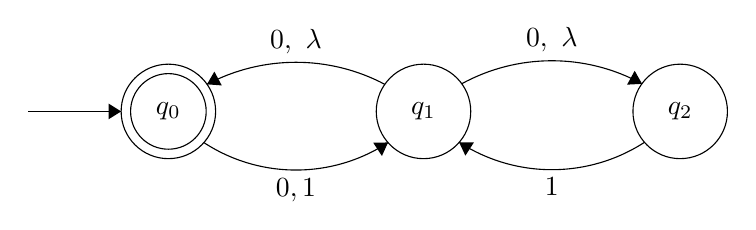
\begin{tikzpicture}[scale=0.2]
            \tikzstyle{every node}+=[inner sep=0pt]
            \draw [black] (13.5,-29.5) circle (3);
            \draw (13.5,-29.5) node {$q_0$};
            \draw [black] (13.5,-29.5) circle (2.4);
            \draw [black] (29.7,-29.5) circle (3);
            \draw (29.7,-29.5) node {$q_1$};
            \draw [black] (46,-29.5) circle (3);
            \draw (46,-29.5) node {$q_2$};
            \draw [black] (4.6,-29.5) -- (10.5,-29.5);
            \fill [black] (10.5,-29.5) -- (9.7,-29) -- (9.7,-30);
            \draw [black] (27.454,-31.474) arc (-56.73531:-123.26469:10.673);
            \fill [black] (27.45,-31.47) -- (26.51,-31.49) -- (27.06,-32.33);
            \draw (21.6,-33.72) node [below] {$0,1$};
            \draw [black] (15.951,-27.783) arc (117.899:62.101:12.074);
            \fill [black] (15.95,-27.78) -- (16.89,-27.85) -- (16.42,-26.97);
            \draw (21.6,-25.88) node [above] {$0,\mbox{ }\lambda$};
            \draw [black] (32.124,-27.746) arc (118.68171:61.31829:11.93);
            \fill [black] (43.58,-27.75) -- (43.11,-26.92) -- (42.63,-27.8);
            \draw (37.85,-25.78) node [above] {$0,\mbox{ }\lambda$};
            \draw [black] (43.74,-31.458) arc (-57.03314:-122.96686:10.824);
            \fill [black] (31.96,-31.46) -- (32.36,-32.31) -- (32.9,-31.47);
            \draw (37.85,-33.7) node [below] {$1$};
        \end{tikzpicture}
    \end{center}

    \begin{itemize}
        \item What is $\delta^*(q_0, 01)$?
        \item Is 01 accepted by this NFA?
        \item What is the language accepted by this NFA?
    \end{itemize}

\end{frame}

\begin{frame}[t]{Exercise}
    \textbf{Exercise.}  Create an NFA that accepts the language $\{xwx : x \in \{0, 1\}, w \in \{0, 1\}^*\}$.

\end{frame}

\section{NFA-to-DFA}

\begin{frame}{NFA-to-DFA}

\end{frame}

\begin{frame}{NFA-to-DFA Algorithm}
    Given an NFA $N = (Q, \Sigma, \delta, q_0, F)$, how can we convert it to a DFA $M = (Q', \Sigma, \delta', S_0, F')$ such that $L(N) = L(M)$?

    Procedure:
    \begin{enumerate}[Step 1: ]
        \item Create an initial state $S_0$. Assign it to $\{q_0\}$.
        \item For each symbol $a \in \Sigma$, find all the states in $N$ that can be reached from each of the states in $S_0$. The set of reachable states in $N$ will become a state in $M$ i.e. $\delta'(S, a) = \underset{p \in S_0}\bigcup\delta(p,a)$.
        \item Repeat Step 2 on every new state $S$ (which are \textit{sets} of states of $N$) that is generated. Repeat until no new states are found.
        \item Assign $Q'$ to the set of states generated in Step 3. $\delta'$ is defined as above.
    \end{enumerate}
    The initial state for the DFA will be $S_0 \coloneqq \{q_0\}$. The final states of the DFA will be all those states $S$ that contain a final state from $F$ (from the original $N$). Finally, if the original NFA $N$ accepts $\lambda$, make $S_0$ a final state.
\end{frame}

\begin{frame}{Example}
    \textbf{Example.} Consider the following NFA $N$. $\Sigma = \{0, 1\}$. What is the language accepted by $N$?
    \begin{center}
        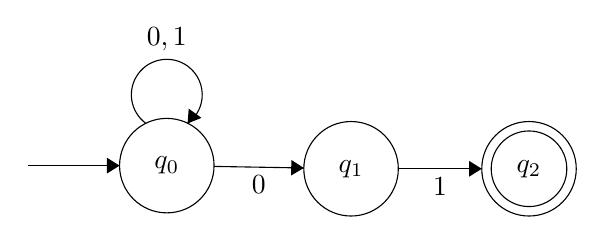
\begin{tikzpicture}[scale=0.2]
            \tikzstyle{every node}+=[inner sep=0pt]
            \draw [black] (19.1,-20.9) circle (3);
            \draw (19.1,-20.9) node {$q_0$};
            \draw [black] (30.8,-21.1) circle (3);
            \draw (30.8,-21.1) node {$q_1$};
            \draw [black] (42.1,-21.1) circle (3);
            \draw (42.1,-21.1) node {$q_2$};
            \draw [black] (42.1,-21.1) circle (2.4);
            \draw [black] (10.3,-20.9) -- (16.1,-20.9);
            \fill [black] (16.1,-20.9) -- (15.3,-20.4) -- (15.3,-21.4);
            \draw [black] (17.777,-18.22) arc (234:-54:2.25);
            \draw (19.1,-13.65) node [above] {$0,1$};
            \fill [black] (20.42,-18.22) -- (21.3,-17.87) -- (20.49,-17.28);
            \draw [black] (22.1,-20.95) -- (27.8,-21.05);
            \fill [black] (27.8,-21.05) -- (27.01,-20.54) -- (26.99,-21.53);
            \draw (24.94,-21.52) node [below] {$0$};
            \draw [black] (33.8,-21.1) -- (39.1,-21.1);
            \fill [black] (39.1,-21.1) -- (38.3,-20.6) -- (38.3,-21.6);
            \draw (36.45,-21.6) node [below] {$1$};
        \end{tikzpicture}
    \end{center}
\end{frame}

\begin{frame}{Example}
    \textbf{Example.} Convert the NFA $N$ to a DFA $M$ such that $L(N) = L(M)$.
    \begin{center}
        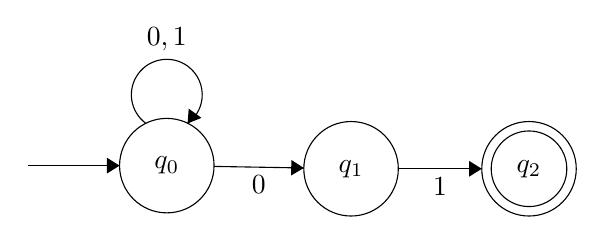
\begin{tikzpicture}[scale=0.2]
            \tikzstyle{every node}+=[inner sep=0pt]
            \draw [black] (19.1,-20.9) circle (3);
            \draw (19.1,-20.9) node {$q_0$};
            \draw [black] (30.8,-21.1) circle (3);
            \draw (30.8,-21.1) node {$q_1$};
            \draw [black] (42.1,-21.1) circle (3);
            \draw (42.1,-21.1) node {$q_2$};
            \draw [black] (42.1,-21.1) circle (2.4);
            \draw [black] (10.3,-20.9) -- (16.1,-20.9);
            \fill [black] (16.1,-20.9) -- (15.3,-20.4) -- (15.3,-21.4);
            \draw [black] (17.777,-18.22) arc (234:-54:2.25);
            \draw (19.1,-13.65) node [above] {$0,1$};
            \fill [black] (20.42,-18.22) -- (21.3,-17.87) -- (20.49,-17.28);
            \draw [black] (22.1,-20.95) -- (27.8,-21.05);
            \fill [black] (27.8,-21.05) -- (27.01,-20.54) -- (26.99,-21.53);
            \draw (24.94,-21.52) node [below] {$0$};
            \draw [black] (33.8,-21.1) -- (39.1,-21.1);
            \fill [black] (39.1,-21.1) -- (38.3,-20.6) -- (38.3,-21.6);
            \draw (36.45,-21.6) node [below] {$1$};
        \end{tikzpicture}
    \end{center}
\end{frame}

\begin{frame}{Example}
    \textbf{Example.} Converting the NFA $N$ to a DFA $M$ using the procedure presented above.
    \begin{enumerate}[Step 1.]
        \item Begin with the start state $S_0 \coloneqq \{q_0\}$.
        \item Find all the states that can be reached from $S_0$ for each letter in $\Sigma$. $\delta'(S_0,0) = \underbrace{\{q_0, q_1\}}_{\text{\textcolor{red}{New state!}}}$, $\delta'(S_0,1) = \{q_0\}$
    \end{enumerate}
    \begin{center}
        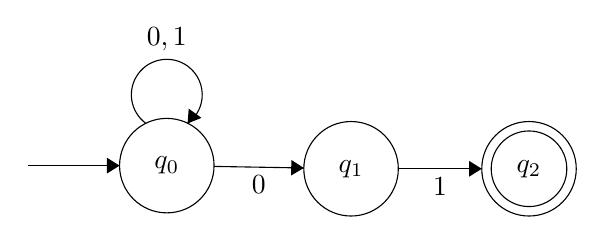
\begin{tikzpicture}[scale=0.2]
            \tikzstyle{every node}+=[inner sep=0pt]
            \draw [black] (19.1,-20.9) circle (3);
            \draw (19.1,-20.9) node {$q_0$};
            \draw [black] (30.8,-21.1) circle (3);
            \draw (30.8,-21.1) node {$q_1$};
            \draw [black] (42.1,-21.1) circle (3);
            \draw (42.1,-21.1) node {$q_2$};
            \draw [black] (42.1,-21.1) circle (2.4);
            \draw [black] (10.3,-20.9) -- (16.1,-20.9);
            \fill [black] (16.1,-20.9) -- (15.3,-20.4) -- (15.3,-21.4);
            \draw [black] (17.777,-18.22) arc (234:-54:2.25);
            \draw (19.1,-13.65) node [above] {$0,1$};
            \fill [black] (20.42,-18.22) -- (21.3,-17.87) -- (20.49,-17.28);
            \draw [black] (22.1,-20.95) -- (27.8,-21.05);
            \fill [black] (27.8,-21.05) -- (27.01,-20.54) -- (26.99,-21.53);
            \draw (24.94,-21.52) node [below] {$0$};
            \draw [black] (33.8,-21.1) -- (39.1,-21.1);
            \fill [black] (39.1,-21.1) -- (38.3,-20.6) -- (38.3,-21.6);
            \draw (36.45,-21.6) node [below] {$1$};
        \end{tikzpicture}
    \end{center}
\end{frame}

\begin{frame}{Example}
    \begin{enumerate}[Step 3.]
        \item Repeat Step 2 on every new state that is generated. Repeat until no new states are produced. This is shown in the table below.
    \end{enumerate}
    \begin{center}
        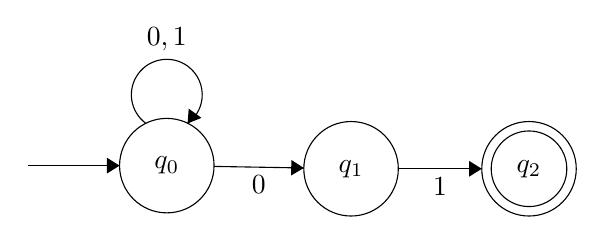
\begin{tikzpicture}[scale=0.2]
            \tikzstyle{every node}+=[inner sep=0pt]
            \draw [black] (19.1,-20.9) circle (3);
            \draw (19.1,-20.9) node {$q_0$};
            \draw [black] (30.8,-21.1) circle (3);
            \draw (30.8,-21.1) node {$q_1$};
            \draw [black] (42.1,-21.1) circle (3);
            \draw (42.1,-21.1) node {$q_2$};
            \draw [black] (42.1,-21.1) circle (2.4);
            \draw [black] (10.3,-20.9) -- (16.1,-20.9);
            \fill [black] (16.1,-20.9) -- (15.3,-20.4) -- (15.3,-21.4);
            \draw [black] (17.777,-18.22) arc (234:-54:2.25);
            \draw (19.1,-13.65) node [above] {$0,1$};
            \fill [black] (20.42,-18.22) -- (21.3,-17.87) -- (20.49,-17.28);
            \draw [black] (22.1,-20.95) -- (27.8,-21.05);
            \fill [black] (27.8,-21.05) -- (27.01,-20.54) -- (26.99,-21.53);
            \draw (24.94,-21.52) node [below] {$0$};
            \draw [black] (33.8,-21.1) -- (39.1,-21.1);
            \fill [black] (39.1,-21.1) -- (38.3,-20.6) -- (38.3,-21.6);
            \draw (36.45,-21.6) node [below] {$1$};
        \end{tikzpicture}
    \end{center}
    \begin{table}[]
        \begin{tabular}{|c|cc|}
            \hline
            States $S$     & $\underset{p \in S}\bigcup\delta(p,0)$ & $\underset{p \in S}\bigcup\delta(p,1)$ \\ \hline
            $\{q_0\}$      & $\{q_0, q_1\}$                         & $\{q_0\}$                              \\ \hline
            $\{q_0, q_1\}$ & $\{q_0, q_1\}$                         & $\{q_0, q_2\}$                         \\ \hline
            $\{q_0, q_2\}$ & $\{q_0, q_1\}$                         & $\{q_0\}$                              \\ \hline
        \end{tabular}
    \end{table}
\end{frame}

\begin{frame}{Example}
    \begin{enumerate}[Step 4.]
        \item Build the DFA.
    \end{enumerate}
    \begin{table}[]
        \begin{tabular}{|c|cc|}
            \hline
            States $S$     & $\delta'(S, 0)$ & $\delta'(S, 1)$ \\ \hline
            $\{q_0\}$      & $\{q_0, q_1\}$  & $\{q_0\}$       \\ \hline
            $\{q_0, q_1\}$ & $\{q_0, q_1\}$  & $\{q_0, q_2\}$  \\ \hline
            $\{q_0, q_2\}$ & $\{q_0, q_1\}$  & $\{q_0\}$       \\ \hline
        \end{tabular}
    \end{table}
    \begin{center}
        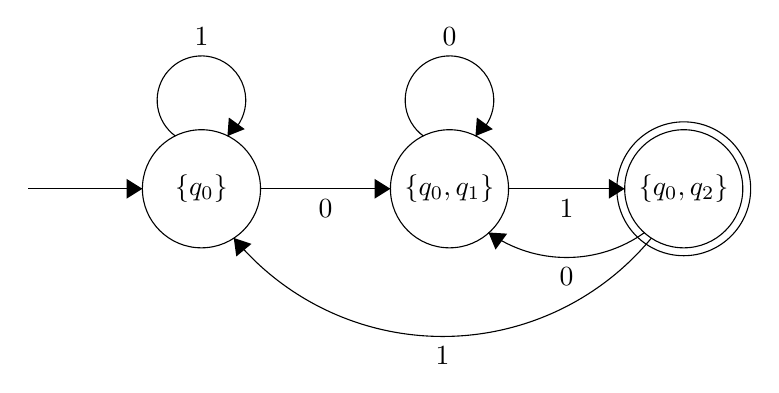
\begin{tikzpicture}[scale=0.25]
            \tikzstyle{every node}+=[inner sep=0pt]
            \draw [black] (18.9,-21.1) circle (3);
            \draw (18.9,-21.1) node {$\{q_0\}$};
            \draw [black] (31.5,-21.1) circle (3);
            \draw (31.5,-21.1) node {$\{q_0,q_1\}$};
            \draw [black] (43.4,-21.1) circle (3.4);
            \draw (43.4,-21.1) node {$\{q_0,q_2\}$};
            \draw [black] (43.4,-21.1) circle (3);
            \draw [black] (10.1,-21.1) -- (15.9,-21.1);
            \fill [black] (15.9,-21.1) -- (15.1,-20.6) -- (15.1,-21.6);
            \draw [black] (17.577,-18.42) arc (234:-54:2.25);
            \draw (18.9,-13.85) node [above] {$1$};
            \fill [black] (20.22,-18.42) -- (21.1,-18.07) -- (20.29,-17.48);
            \draw [black] (21.9,-21.1) -- (28.5,-21.1);
            \fill [black] (28.5,-21.1) -- (27.7,-20.6) -- (27.7,-21.6);
            \draw (25.2,-21.6) node [below] {$0$};
            \draw [black] (34.5,-21.1) -- (40.4,-21.1);
            \fill [black] (40.4,-21.1) -- (39.6,-20.6) -- (39.6,-21.6);
            \draw (37.45,-21.6) node [below] {$1$};
            \draw [black] (41.416,-23.318) arc (-54.41125:-125.58875:6.816);
            \fill [black] (33.48,-23.32) -- (33.84,-24.19) -- (34.43,-23.38);
            \draw (37.45,-25.09) node [below] {$0$};
            \draw [black] (30.177,-18.42) arc (234:-54:2.25);
            \draw (31.5,-13.85) node [above] {$0$};
            \fill [black] (32.82,-18.42) -- (33.7,-18.07) -- (32.89,-17.48);
            \draw [black] (41.757,-23.603) arc (-39.52969:-140.47031:13.752);
            \fill [black] (20.54,-23.6) -- (20.67,-24.54) -- (21.44,-23.9);
            \draw (31.15,-29.1) node [below] {$1$};
        \end{tikzpicture}
    \end{center}
\end{frame}

\begin{frame}{Exercise}
    \textbf{Exercise.} Convert the following NFA $N$ into an equivalent DFA $M$. Your conversion should ensure that $L(N) = L(M)$. $\Sigma = \{a, b\}$.
    \begin{center}
        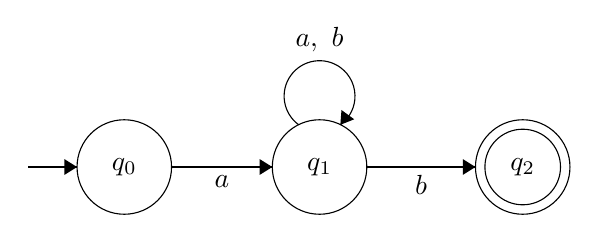
\begin{tikzpicture}[scale=0.2]
        \tikzstyle{every node}+=[inner sep=0pt]
        \draw [black] (25.5,-27.6) circle (3);
        \draw (25.5,-27.6) node {$q_0$};
        \draw [black] (37.9,-27.6) circle (3);
        \draw (37.9,-27.6) node {$q_1$};
        \draw [black] (50.8,-27.6) circle (3);
        \draw (50.8,-27.6) node {$q_2$};
        \draw [black] (50.8,-27.6) circle (2.4);
        \draw [black] (28.5,-27.6) -- (34.9,-27.6);
        \fill [black] (34.9,-27.6) -- (34.1,-27.1) -- (34.1,-28.1);
        \draw (31.7,-28.1) node [below] {$a$};
        \draw [black] (19.4,-27.6) -- (22.5,-27.6);
        \fill [black] (22.5,-27.6) -- (21.7,-27.1) -- (21.7,-28.1);
        \draw [black] (36.577,-24.92) arc (234:-54:2.25);
        \draw (37.9,-20.35) node [above] {$a,\mbox{ }b$};
        \fill [black] (39.22,-24.92) -- (40.1,-24.57) -- (39.29,-23.98);
        \draw [black] (40.9,-27.6) -- (47.8,-27.6);
        \fill [black] (47.8,-27.6) -- (47,-27.1) -- (47,-28.1);
        \draw (44.35,-28.1) node [below] {$b$};
        \end{tikzpicture}
    \end{center}
\end{frame}

\begin{frame}{Theorem}
    \textbf{Theorem.} The set of all languages accepted by NFAs is the same as the set of all languages accepted by DFAs.\\
    Why?
    \begin{enumerate}[1.]
        \item Every DFA is an NFA.
        \item Every NFA can be converted into a DFA.
    \end{enumerate}
    \textbf{Corollary.} A language is regular if and only if there is an FA (either a DFA or NFA) that accepts it.
\end{frame}

\begin{frame}[t]{Exercise}
    \textbf{Exercise.}  Prove that the language $\{xwx : x \in \{0, 1\}, w \in \{0, 1\}^*\}$ is regular.

\end{frame}


\end{document}





